\documentclass[a4paper,12pt]{article}

%% ── Encoding & Language ──────────────────────────────────────────────────────
\usepackage[utf8]{inputenc}
\usepackage[T1]{fontenc}
\usepackage[english]{babel}

%% ── Fonts & Spacing ──────────────────────────────────────────────────────────
\renewcommand{\rmdefault}{ptm}
\usepackage{palatino}
\usepackage{mathpazo}
\usepackage{lmodern}
\usepackage{setspace}
\onehalfspacing
\usepackage{parskip}
\interfootnotelinepenalty=10000

%% ── Page Layout ──────────────────────────────────────────────────────────────
\usepackage[top=.75in, bottom=1in, right=.9in, left=.9in]{geometry}
\usepackage{pdflscape}
\usepackage{titling}

%% ── Math ─────────────────────────────────────────────────────────────────────
\usepackage{amsmath,amssymb,amsfonts,amsthm}
\usepackage{bm}
\usepackage{eurosym}
\usepackage{siunitx}

%% ── Graphics & Figures ───────────────────────────────────────────────────────
\usepackage[pdftex]{graphicx}
\usepackage{subcaption}
\usepackage[capposition=top]{floatrow}

%% ── Tables ───────────────────────────────────────────────────────────────────
\usepackage{booktabs}
\usepackage{multirow}
\usepackage{array}
\usepackage{adjustbox}
\usepackage{makecell}
\usepackage[flushleft]{threeparttable}
\usepackage{setspace}
\AtBeginEnvironment{tabular*}{\singlespacing}
\AtBeginEnvironment{tablenotes}{\singlespacing}

%% ── Colors ───────────────────────────────────────────────────────────────────
\usepackage[dvipsnames]{xcolor}
\newcommand{\red}[1]{{\color{red} #1}}
\newcommand{\blue}[1]{{\color{blue} #1}}

%% ── Section Styling ──────────────────────────────────────────────────────────
\usepackage{sectsty}
\sectionfont{\color{BlueViolet}}
\subsectionfont{\color{BlueViolet}}
\usepackage{titlesec}

%% ── Hyperlinks ───────────────────────────────────────────────────────────────
\usepackage[colorlinks=true, citecolor=blue, linkcolor=black, urlcolor=black]{hyperref}
\usepackage{cleveref}

%% ── Bibliography ─────────────────────────────────────────────────────────────
\usepackage{apacite}

%% ── Lists & Misc ─────────────────────────────────────────────────────────────
\usepackage{enumitem}
\usepackage{multicol}
\usepackage{verbatim}
\usepackage{soul}
\usepackage{ragged2e}
\usepackage{footmisc}
\renewcommand{\footnotelayout}{\setstretch{.9}}
\usepackage{endnotes}
\usepackage{pdfpages}
\usepackage[toc,page]{appendix}

%% ── Custom Column Types ──────────────────────────────────────────────────────
\newcolumntype{L}[1]{>{\raggedright\let\newline\\arraybackslash\hspace{0pt}}m{#1}}
\newcolumntype{C}[1]{>{\centering\let\newline\\arraybackslash\hspace{0pt}}m{#1}}
\newcolumntype{R}[1]{>{\raggedleft\let\newline\\arraybackslash\hspace{0pt}}m{#1}}

%% ── Theorem Environments ─────────────────────────────────────────────────────
\newtheorem{theorem}{Theorem}
\newtheorem{corollary}[theorem]{Corollary}
\newtheorem{proposition}{Proposition}
\newtheorem{hyp}{Hypothesis}
\newtheorem{subhyp}{Hypothesis}[hyp]
\renewcommand{\thesubhyp}{\thehyp\alph{subhyp}}
\begin{document}

\begin{titlepage}
\title{When Tradable Inflation Becomes Domestic: Second-Round Effects and Monetary Policy Trade-Offs\thanks{We thank participants at the meetings of the ...}}
\author{Mananirina Razafitsiory \thanks{Department of Economics, Pavillon J.-A.-DeS\`eve, 1025, avenue des Sciences-Humaines, Universit\'e Laval, Qu\'ebec (Qu\'ebec) G1V 0A6, Canada.  Email: \url{mananirina.razafitsiory.1@ulaval.ca}.
} and Zo Andriantomanga \thanks{Department of Economics, 2442 E. Kenwood Blvd. Milwaukee, WI 53201-0729 United States University of Wisconsin Milwaukee.  Email:\url{andrian2@uwm.edu}}
}

\date{\today}
\maketitle
\begin{abstract}
\noindent Appendix \\
\vspace{0in}\\
\noindent\textbf{Keywords:} key1, key2, key3\\
\vspace{0in}\\
\noindent\textbf{JEL Codes:} key1, key2, key3\\

\bigskip
\end{abstract}
\setcounter{page}{0}
\thispagestyle{empty}
\end{titlepage}
\pagebreak \newpage




\doublespacing


%%%%%%%%%%%%%%%%%%%%%%%%%%%%%%%%%%%%%%%%%%%%%%%%%%%%%%%%%%%%%%%%%%%%%%%%%%%%%%%%%%%%%%%%%%%%%%%%%%%%%%%%%%%%%%%%%%%%%%%%%%%%%%%%%%%%%%%%%%%%%%%%%%%
%%%%%%%%%%%%%%%%%%%%%%%%%%%%%%%%%%%%%%%%%%%%%%%%%%%%%%%%%%%%%%%%%%%%%%%%%%%%%%%%%%%%%%%%%%%%%%%%%%%%%%%%%%%%%%%%%%%%%%%%%%%%%%%%%%%%%%%%%%%%%%%%%%%
%%%%%%%%%%%%%%%%%%%%%%%%%%%%%%%%%%%%%%%%%%%%%%%%%%%%%%%%%%%%%%%%%%%%%%%%%%%%%%%%%%%%%%%%%%%%%%%%%%%%%%%%%%%%%%%%%%%%%%%%%%%%%%%%%%%%%%%%%%%%%%%%%%%
%%%%%%%%%%%%%%%%%%%%%%%%%%%%%%%%%%%%%%%%%%%%%%%%%%%%%%%%%%%%%%%%%%%%%%%%%%%%%%%%%%%%%%%%%%%%%%%%%%%%%%%%%%%%%%%%%%%%%%%%%%%%%%%%%%%%%%%%%%%%%%%%%%%
%%%%%%%%%%%%%%%%%%%%%%%%%%%%%%%%%%%%%%%%%%%%%%%%%%%%%%%%%%%%%%%%%%%%%%%%%%%%%%%%%%%%%%%%%%%%%%%%%%%%%%%%%%%%%%%%%%%%%%%%%%%%%%%%%%%%%%%%%%%%%%%%%%%
%%%%%%%%%%%%%%%%%%%%%%%%%%%%%%%%%%%%%%%%%%%%%%%%%%%%%%%%%%%%%%%%%%%%%%%%%%%%%%%%%%%%%%%%%%%%%%%%%%%%%%%%%%%%%%%%%%%%%%%%%%%%%%%%%%%%%%%%%%%%%%%%%%%
%%%%%%%%%%%%%%%%%%%%%%%%%%%%%%%%%%%%%%%%%%%%%%%%%%%%%%%%%%%%%%%%%%%%%%%%%%%%%%%%%%%%%%%%%%%%%%%%%%%%%%%%%%%%%%%%%%%%%%%%%%%%%%%%%%%%%%%%%%%%%%%%%%%
%%%%%%%%%%%%%%%%%%%%%%%%%%%%%%%%%%%%%%%%%%%%%%%%%%%%%%%%%%%%%%%%%%%%%%%%%%%%%%%%%%%%%%%%%%%%%%%%%%%%%%%%%%%%%%%%%%%%%%%%%%%%%%%%%%%%%%%%%%%%%%%%%%%
%%%%%%%%%%%%%%%%%%%%%%%%%%%%%%%%%%%%%%%%%%%%%%%%%%%%%%%%%%%%%%%%%%%%%%%%%%%%%%%%%%%%%%%%%%%%%%%%%%%%%%%%%%%%%%%%%%%%%%%%%%%%%%%%%%%%%%%%%%%%%%%%%%%
%%%%%%%%%%%%%%%%%%%%%%%%%%%%%%%%%%%%%%%%%%%%%%%%%%%%%%%%%%%%%%%%%%%%%%%%%%%%%%%%%%%%%%%%%%%%%%%%%%%%%%%%%%%%%%%%%%%%%%%%%%%%%%%%%%%%%%%%%%%%%%%%%%%
%%%%%%%%%%%%%%%%%%%%%%%%%%%%%%%%%%%%%%%%%%%%%%%%%%%%%%%%%%%%%%%%%%%%%%%%%%%%%%%%%%%%%%%%%%%%%%%%%%%%%%%%%%%%%%%%%%%%%%%%%%%%%%%%%%%%%%%%%%%%%%%%%%%
%%%%%%%%%%%%%%%%%%%%%%%%%%%%%%%%%%%%%%%%%%%%%%%%%%%%%%%%%%%%%%%%%%%%%%%%%%%%%%%%%%%%%%%%%%%%%%%%%%%%%%%%%%%%%%%%%%%%%%%%%%%%%%%%%%%%%%%%%%%%%%%%%%%
%%%%%%%%%%%%%%%%%%%%%%%%%%%%%%%%%%%%%%%%%%%%%%%%%%%%%%%%%%%%%%%%%%%%%%%%%%%%%%%%%%%%%%%%%%%%%%%%%%%%%%%%%%%%%%%%%%%%%%%%%%%%%%%%%%%%%%%%%%%%%%%%%%%
%%%%%%%%%%%%%%%%%%%%%%%%%%%%%%%%%%%%%%%%%%%%%%%%%%%%%%%%%%%%%%%%%%%%%%%%%%%%%%%%%%%%%%%%%%%%%%%%%%%%%%%%%%%%%%%%%%%%%%%%%%%%%%%%%%%%%%%%%%%%%%%%%%%
%%%%%%%%%%%%%%%%%%%%%%%%%%%%%%%%%%%%%%%%%%%%%%%%%%%%%%%%%%%%%%%%%%%%%%%%%%%%%%%%%%%%%%%%%%%%%%%%%%%%%%%%%%%%%%%%%%%%%%%%%%%%%%%%%%%%%%%%%%%%%%%%%%%
%%%%%%%%%%%%%%%%%%%%%%%%%%%%%%%%%%%%%%%%%%%%%%%%%%%%%%%%%%%%%%%%%%%%%%%%%%%%%%%%%%%%%%%%%%%%%%%%%%%%%%%%%%%%%%%%%%%%%%%%%%%%%%%%%%%%%%%%%%%%%%%%%%%
% %%%%%%%%%%%%%%%%%%%%%%%%%%%%%%%%%%%%%%%%%%%%%%%%%%%%%%%%%%
% %%%%%%%%%%%%%%%%%%%%%%%%%%%%%%%%%%%%%%%%%%%%%%%%%%%%%%%%%%
% BODY OF THE DOCUMENT
% %%%%%%%%%%%%%%%%%%%%%%%%%%%%%%%%%%%%%%%%%%%%%%%%%%%%%%%%%%
% %%%%%%%%%%%%%%%%%%%%%%%%%%%%%%%%%%%%%%%%%%%%%%%%%%%%%%%%%%
%%%%%%%%%%%%%%%%%%%%%%%%%%%%%%%%%%%%%%%%%%%%%%%%%%%%%%%%%%%%%%%%%%%%%%%%%%%%%%%%%%%%%%%%%%%%%%%%%%%%%%%%%%%%%%%%%%%%%%%%%%%%%%%%%%%%%%%%%%%%%%%%%%%%%%%%%%%%%%%%%%%%%%%%%%%%%%%%%%%%%%%%%%%%%%%%%%%%%%%%%%%%%%%%%%%%%%%%%%%%%%%%%%%%%%%%%%%%%%%%%%%%%%%%%%%%%%%%%%%%%%%%%%%%%%%%%%%%%%%%%%%%%%%%%%%%%%%%%%%%%%%%%%%%%%%%%%%%%%%%%%%%%%%%%%%%%%%%%%%%%%%%%%%%%%%%%%%%%%%%%%%%%%%%%%%%%%%%%%%%%%%%%%%%%%%%%%%%%%%%%%%%%%%%%%%%%%%%%%%%%%%%%%%%%%%%%%%%%%%%%%%%%%%%%%%%%%%%%%%%%%%%%%%%%%%%%%%%%%%%%%%%%%%%%%%%%%%%%%%%%%%%%%%%%%%%%%%%%%%%%%%%%%%%%%%%%%%%%%%%%%%%%%%%%%%%%%%%%%%%%%%%%%%%%%%%%%%%%%%%%%%%%%%%%%%%%%%%%%%%%%%%%%%%%%%%%%%%%%%%%%%%%%%%%%%%%%%%%%%%%%%%%%%%%%%%%%%%%%%%%%%%%%%%%%%%%%%%%%%%%%%%%%%%%%%%%%%%%%%%%%%%%%%%%%%%%%%%%%%%%%%%%%%%%%%%%%%%%%%%%%%%%%%%%%%%%%%%%%%%%%%%%%%%%%%%%%%%%%%%%%%%%%%%%%%%%%%%%%%%%%%%%%%%%%%%%%%%%%%%%%%%%%%%%%%%%%%%%%%%%%%%%%%%%%%%%%%%%%%%%%%%%%%%%%%%%%%%%%%%%%%%%%%%%%%%%%%%%%%%%%%%%%%%%%%%%%%%%%%%%%%%%%%%%%%%%%%%%%%%%%%%%%%%%%%%%%%%%%%%%%%%%%%%%%%%%%%%%%%%%%%%%%%%%%%%%%%%%%%%%%%%%%%%%%%%%%%%%%%%%%%%%%%%%%%%%%%%%%%%%%%%%%%%%%%%%%%%%%%%%%%%%%%%%%%%%%%%%%%%%%%%%%%%%%%%%%%%%%%%%%%%%%%%%%%%%%%%%%%%%%%%%%%%%%%%%%%%%%%%%%%%%%%%%%%%%%%%%%%%%%%%%%%%%%%%%%%%%%%%%%%%%%%%%%%%%%%%%%%%%%%%%%%%%%%%%%%%%%%%%%%%%%%%%%%%%%%%%%%%%%%%%%%%%%%%%%%%%%%%%%%%%%%%%%%%%%%%%%%%%%%%%%%%%%%%%%%%%%%%%%%%%%%%%%%%%%%%%%%%%%%%%%%%%%%%%%%%%%%%%%%%%%%%%%%%%%%%%%%%%%%%%%%%%%%%%%%%%%%%%%%%%%%%%%%%%%%%%%%%%%%%%%%%%%%%%%%%%%%%%%%%%%%%%%%%%%%%%%%%%%%%%%%%%%%%%%%%%%%%%%%%%%%%%%%%%%%%%%%%%%%%%%%%%%%%%%%%%%%%%%%%%%%%%%%%%%%%%%%%%%%%%%%%%%%%%%%%%%%%%%%%%%%%%%%%%%%%%%%%%%%%%%%%%%%%%%%%%%%%%%%%%%%%%%%%%%%%%%%%%%%%%%%%%%%%%%%%%%%%%%%%%%%%%%%%%%%%%%%%%%%%%%%%%%%%%%%%%%%%%%%%%%%%%%%%%%%%%%%%%%%%%%%%%%%%%%%%%%%%%%%%%%%%%%%%%%%%%%%%%%%%%%%%%%%%%%%%%%%%%%%%%%%%%%%%%%%%%%%%%%%%%%%%%%%%%%%%%%%%%%%%%%%%%%%%%%%%%%%%%%%%%%%%%%%%%%%%%%%%%%%%%%%%%%%%%%%%%%%%%%%%%%%%%%%%%%%%%%%%%%%%%%%%%%%%%%%%%%%%%%%%%%%%%%%%%%%%%%%%%%%%%%%%%%%%%%%%%%%%%%%%%%%%%%%%%%%%%%%%%%%%%%%%%%%%%%%%%%%%%%%%%%%%%%%%%%%%%%%%%%%%%%%%%%%%%%%%%%%%%%%%%%%%%%%%%%%%%%%%%%%%%%%%%%%%%%%%%%%%%%%%%%%%%%%%%%%%%%%%%%%%%%%%%%%%%%%%%%%%%%%%%%%%%%%%%%%%%%%%%%%%%%%%%%%%%%%%%%%%%%%%%%%%%%%%%%%%%%%%%%%%%%%%%%%%%%%%%%%%%%%%%%%%%%%%%%%%%%%%%%%%%%%%%%%%%%%%%%%%%%%%%%%%%%%%%%%%%%%%%%%%%%%%%%%%%%%%%%%%%%%%%%%%%%%%%%%%%%%%%%%%%%%%%%%%%%%%%%%%%%%%%%%%%%%%%%%%%%%%%%%%%%%%%%%%%%%%%%%%%%%%%%%%%%%%%%%%%%%%%%%%%%%%%%%%%%%%%%%%%%%%%%%%%%%%%%%%%%%%%%%%%%%%%%%%%%%%%%%%%%%%%%%%%%%%%%%%%%%%%%%%%%%%%%%%%%%%%%%%%%%%%%%%%%%%%%%%%%%%%%%%%%%%%%%%%%%%%%%%%%%%%%%%%%%%%%%%%%%%%%%%%%%%%%%%%%%%%%%%%%%%%%%%%%%%%%%%%%%%%%%%%%%%%%%%%%%%%%%%%%%%%%%%%%%%%%%%%%%%%%%%%%%%%%%%%%%%%%%%%%%%%%%%%%%%%%%%%%%%%%%%%%%%%%%%%%%%%%%%%%%%%%%%%%%%%%%%%%%%%%%%%%%%%%%%%%%%%%%%%%%%%%%%%%%%%%%%%%%%%%%%%%%%%%%%%%%%%%%%%%%%%%%%%%%%%%%%%%%%%%%%%%%%%%%%%%%%%%%%%%%%%%%%%%%%%%%%%%%%%%%%


% %%%%%%%%%%%%%%%%%%%%%%%%%%%%%%%%%%%%%%%%%%%%%%%%%%%%%%%%%%
% %%%%%%%%%%%%%%%%%%%%%%%%%%%%%%%%%%%%%%%%%%%%%%%%%%%%%%%%%%
% INTRODUCTION
% %%%%%%%%%%%%%%%%%%%%%%%%%%%%%%%%%%%%%%%%%%%%%%%%%%%%%%%%%%
% %%%%%%%%%%%%%%%%%%%%%%%%%%%%%%%%%%%%%%%%%%%%%%%%%%%%%%%%%%

\section{Introduction}


The post-pandemic inflation episode in the euro area was remarkable not only for its initial severity but for its persistence. Leading explanations in the literature point to demand-side pressures from fiscal stimulus and the pandemic-era reallocation of household expenditure, supply-chain disruptions that constrained the production of manufactured goods, and large shocks to energy and food prices \cite{BernankeBlanchardAEJM, DaoGourinchasLeighMishra2024}. These accounts are well-grounded, yet they share a common limitation: they treat the initial shock as the primary object of interest and leave underexplored the domestic propagation mechanism that determined how long that shock remained embedded in prices. This paper argues that a complementary mechanism was central to the persistence of the episode: strong second-round pass-through from tradable to non-tradable inflation.

Second-round pass-through is the process by which an initial increase in the prices of traded goods propagates into the prices of services and other non-tradable goods. When this channel is weak, an imported cost shock is largely a relative price shift: it raises headline inflation temporarily but leaves the domestic wage and price-setting process undisturbed. When it is strong, the same shock activates domestic inflation dynamics, generates persistence, and alters the trade-offs facing monetary policy in a fundamental way. The policy question is then not only what caused the original shock but whether and how quickly it became embedded in the domestic prices that are directly relevant for the ECB's inflation target.

This paper studies the dynamic causal pass-through from tradable to non-tradable inflation in a monthly panel of 20 euro area countries from January 1998 to December 2025. The European Monetary Union is the natural laboratory for this question. The common monetary policy and shared exchange rate remove the confounding variation in policy responses that complicates cross-country comparisons: differences in pass-through across member states reflect genuine variation in structural conditions rather than differential interest rate or exchange rate reactions. At the same time, the EMU's institutional design creates a specific and consequential policy problem. The ECB sets a single interest rate for economies that differ substantially in how imported cost shocks propagate into domestic prices. When second-round pass-through is strong in some member states and weak in others, the common stance will be systematically mis-calibrated, too accommodative where amplification is strong and unnecessarily tight where the domestic price-setting process is more insulated. Measuring and understanding this heterogeneity is therefore a precondition for evaluating the welfare costs of asymmetric inflation dynamics inside the union.

Our central data contribution is a new monthly panel of disaggregated HICP components with time-varying ECOICOP expenditure weights, which allows us to construct tradable and non-tradable inflation directly from consumer price data rather than relying on producer prices or import prices as proxies, as much of the existing literature does \citeA{HaKoseOhnsorge2023}. The tradable expenditure share of each country's CPI basket varies across both countries and time, and this variation is the foundation of our identification strategy.

Identification proceeds through a panel local projection instrumental variables (LP-IV) estimator in which tradable inflation is instrumented by a Bartik shift-share $Z_{it} = w_{it} \cdot \varepsilon_t$, where $w_{it}$ is the country-time-varying tradables expenditure share and $\varepsilon_t$ is the market-based oil price expectation shock of \citeA{BaumeisterHamilton2019}. The shift-share structure means that the same common oil price impulse generates heterogeneous variation in tradable inflation across countries through differences in basket composition, providing identifying variation that is orthogonal to country-specific demand conditions. The baseline results are robust across three instrument variants that exploit different sources of cross-country variation.

The baseline LP-IV impulse response of non-tradable inflation to a one-percentage-point increase in instrumented tradable inflation is positive and statistically significant throughout the thirteen-month estimation window, peaking at 0.96 at month six in a double-humped profile consistent with a faster input-cost channel and a slower wage-bargaining channel that re-amplifies the response around month ten. This full-sample average, however, masks substantial variation across regimes and time periods.

The more consequential finding is that this pass-through is not a structural constant. The full-sample estimate of 0.96 conceals a dramatic divergence between the pre-2020 period, where pass-through peaks at 0.48, and the post-2020 period, where it peaks near 1.4; this divergence is the first evidence that pass-through is regime-dependent. Under supply-chain stress, measured by the Global Supply Chain Pressure Index of \shortciteA{BenignodiGiovannietal2022}, peak pass-through nearly triples relative to normal times, rising from below 0.5 to approximately 1.5. The exchange rate dimension produces the sharpest contrast: depreciation episodes generate a peak pass-through of approximately 2.05 at month ten, roughly four times the modest and statistically insignificant response observed during appreciation episodes, indicating that currency movements are a first-order amplifier of second-round effects rather than a channel through which they dissipate. Elevated inflation volatility similarly amplifies pass-through, consistent with high price instability lowering the threshold at which service-sector firms transmit cost shocks into prices. These three conditions, supply-chain disruptions, exchange rate depreciation, and elevated inflation volatility, mutually reinforced one another during the 2021--22 euro area episode, offering a coherent structural account of why domestic service price inflation remained elevated long after energy prices had peaked.

We bring the empirical estimates to bear on monetary policy by interpreting the estimated pass-through as a structural parameter within a two-sector small open economy New Keynesian model. The model allows us to evaluate how the welfare costs of the ECB's one-size-fits-all stance depend on the underlying degree of second-round pass-through across member states. We find that the costs of policy misalignment are convex in the degree of pass-through: applying a rule calibrated to average conditions in a high-pass-through environment is substantially more costly than the symmetric error in a low-pass-through environment, precisely because strong second-round effects generate persistence that a uniform policy stance cannot offset.

The paper most closely related to ours is \citeA{MerendinoMonacelli2025}, who document that the pass-through of energy prices to consumer price inflation is state-dependent and amplified during periods of supply chain uncertainty, using state-dependent local projections and a New Keynesian model with firm-level Bayesian learning. The key distinction is the object we study: \citeA{MerendinoMonacelli2025} focus on the transmission from energy prices to headline consumer inflation, a channel that operates primarily through the tradable sector. We focus on the subsequent step, the propagation from tradable to non-tradable prices, which is the margin that determines whether an imported shock becomes embedded in domestic inflation. The two papers are therefore complementary: theirs identifies the conditions under which energy shocks are amplified into aggregate consumer prices, ours identifies the conditions under which those amplified tradable price movements then feed through into the service price dynamics that are most directly relevant for the ECB's target. More broadly, this paper contributes to the literatures on open-economy inflation pass-through \cite{BursteinGopinath2014, CorsettiDedolaLeduc2008}, second-round inflation dynamics in the euro area \cite{BobeicaJarocinski2019}, the macroeconomic consequences of supply-chain disruptions \cite{AscariBonamSmadu2024, BenignodiGiovannietal2022}, and optimal monetary policy under imported inflation in currency unions \cite{GaliMonacelli2005, FaiaMonacelli2008}.

The remainder of the paper is organized as follows. Section~\ref{sec:data} describes the data construction. Section~\ref{sec:strategy} presents the empirical strategy. Section~\ref{sec:results} reports the baseline pass-through estimates, documents the divergence between pre- and post-2020 sub-periods, identifies the state-dependent amplification mechanism, and examines cross-country heterogeneity across Core, Periphery, and Small Open Economy member states. Section~\ref{sec:model} develops the structural model and policy evaluation. Section~\ref{sec:conclusion} concludes.

% %%%%%%%%%%%%%%%%%%%%%%%%%%%%%%%%%%%%%%%%%%%%%%%%%%%%%%%%%%
% %%%%%%%%%%%%%%%%%%%%%%%%%%%%%%%%%%%%%%%%%%%%%%%%%%%%%%%%%%
% Literature Review
% %%%%%%%%%%%%%%%%%%%%%%%%%%%%%%%%%%%%%%%%%%%%%%%%%%%%%%%%%%
% %%%%%%%%%%%%%%%%%%%%%%%%%%%%%%%%%%%%%%%%%%%%%%%%%%%%%%%%%%
\section{Literature Review}
The propagation of external cost shocks into domestic non-tradable prices so-called second-round effects is central to monetary policy in open economies, yet the empirical literature on this transmission channel lacks causal identification. \citeA{ReisWatson2010} decompose U.S.\ consumer prices into relative-price changes and pure inflation, finding that aggregate relative-price movements driven largely by tradable goods account for most inflation variability, but they do not estimate the causal link from tradable to non-tradable components. \citeA{AltissimoMojonZaffaroni2009} show that heterogeneous propagation of common shocks to euro area services prices is the principal source of aggregate inflation persistence, establishing the non-tradable sector as the locus where transitory cost shocks become persistent price-level shifts. On specific commodity channels, \citeA{Peersman2022} demonstrates that international food price shocks trigger second-round effects in the euro area through wages and inflation expectations, with significant cross-country heterogeneity in the wage response. \citeA{BobeicaJarocinski2019} find that domestic propagation mechanisms not global factors alone explain the euro area's ``missing inflation'' episode of 2012--2014, pointing to internal transmission as a first-order concern. Most recently, \citeA{Andriantomanga2025} documents systematic spillovers from tradable to non-tradable inflation across 40 countries using a TVP-VAR, while the reverse channel remains muted. These studies collectively establish that tradable price shocks feed into services inflation and that this channel drives persistence. However, none provides causal identification of the pass-through coefficient, nor do they construct tradable and non-tradable price indices directly from disaggregated consumer price components rather than relying on coarse goods-versus-services proxies. This paper addresses both limitations.

The debate over the 2021--2023 inflation surge provides further motivation. \citeA{BernankeBlanchardAEJM} attribute the U.S.\ inflation episode primarily to commodity prices and pandemic supply disruptions rather than wage-price spirals, a finding they extend to eleven advanced economies \cite{BernankeBlanchardMulti}. \citeA{Shapiro2024} decomposes PCE inflation into supply- and demand-driven components and concludes that supply factors accounted for more than half of the 2021--2022 rise. For the euro area, \citeA{di2022global} show that sectoral supply bottlenecks and demand shocks, propagating through global production networks, jointly explain the inflation dynamics, while \citeA{BenignodiGiovannietal2022} introduce the Global Supply Chain Pressure Index and document its predictive power for producer and consumer prices. \citeA{Hansenetal2023} decompose euro area price increases and find that import costs and profits not wages accounted for most of the 2022 rise, and \citeA{Alvarezetal2024} confirm that sustained wage-price spirals are historically rare across advanced economies. \citeA{CavalloLippiMiyahara2024} document that large cost shocks accelerate the frequency of price adjustment, generating faster pass-through than time-dependent models predict. What this body of work largely omits is the propagation mechanism from tradable to non-tradable inflation: existing studies identify initial shocks and quantify aggregate effects but do not isolate the second-round channel through which tradable price increases become embedded in services. Our contribution is to estimate this pass-through causally and to show that its state dependence across supply-chain stress, exchange rate, and inflation-volatility regimes explains why euro area inflation proved more persistent than standard models predicted.

A related literature on exchange rate pass-through (ERPT) connects directly to our finding that depreciation generates roughly four times the tradable-to-non-tradable pass-through of appreciation. \citeA{CampaGoldberg2005} provide benchmark estimates of partial short-run ERPT into import prices for 23 OECD countries, while \citeA{GopinathItskhokiRigobon2010} show that currency of invoicing is a first-order determinant: goods priced in dollars exhibit pass-through of roughly 25 percent versus 95 percent for non-dollar-priced goods. The dominant currency paradigm of \citeA{Gopinathetal2020} formalises how dollar exchange rate movements dominate bilateral rates in pass-through regressions. On asymmetry, \citeA{Bussiere2013} finds that large depreciations pass through to G7 trade prices disproportionately, and \citeA{DelattelopezVillavicencio2012} use asymmetric cointegration to show that depreciations transmit to consumer prices significantly more than appreciations a result that linear models mask entirely. \citeA{CarriereSwallowetal2025} extend the analysis to state dependence, documenting amplified pass-through in high-inflation and high-uncertainty regimes. Our paper shows that this asymmetry extends beyond border prices to the second-round channel: depreciation-driven tradable inflation propagates into non-tradable prices far more strongly than appreciation-driven tradable disinflation.

Methodologically, we combine local projections \cite{Jorda2005} with instrumental variables in the LP-IV framework formalised by \citeA{StockWatson2018}, which offers robustness to misspecification advantages over structural VARs \cite{Ramey2016}. Our Bartik shift-share instrument interacts country-specific expenditure weights on tradable HICP components with common euro area component-level price shocks. Identification follows \citeA{GoldsmithPinkhametal2020} and \citeA{Borusyaketal2022}: under the former, validity requires exogeneity of the expenditure shares; under the latter, quasi-random assignment of the price shocks suffices. We exploit oil supply shocks identified following \citeA{BaumeisterHamilton2019} as a component of the shift variation. This design yields plausibly exogenous variation in tradable inflation, enabling the first causal panel estimates of the second-round pass-through to non-tradable prices in the euro area.
% %%%%%%%%%%%%%%%%%%%%%%%%%%%%%%%%%%%%%%%%%%%%%%%%%%%%%%%%%%
% %%%%%%%%%%%%%%%%%%%%%%%%%%%%%%%%%%%%%%%%%%%%%%%%%%%%%%%%%%
% Data
% %%%%%%%%%%%%%%%%%%%%%%%%%%%%%%%%%%%%%%%%%%%%%%%%%%%%%%%%%%
% %%%%%%%%%%%%%%%%%%%%%%%%%%%%%%%%%%%%%%%%%%%%%%%%%%%%%%%%%%

\section{Data}\label{sec:data}

The data consist of a panel of 20 euro area member states observed at monthly frequency from January 1998 to December 2025, assembled from Eurostat and the ECB Data Portal. Data for Croatia are available from January 1999; all remaining members are observed over the full period, yielding 6,720 country-month observations in total. Table~\ref{tab:summary} presents summary statistics. Table~\ref{tab:sources} documents data sources. Table~\ref{tab:coverage} lists country coverage with sample start and end dates and observation counts.

The central data contribution of this paper is the construction of country-specific tradable and non-tradable inflation measures directly from disaggregated HICP components following the European Classification of Individual Consumption according to Purpose (ECOICOP). For each country $i$ and ECOICOP division $j$, price indices are downloaded from Eurostat dataset \texttt{prc\_hicp\_midx} (monthly, index base 2015\,=\,100) and annual expenditure shares from \texttt{prc\_hicp\_inw}. The year-over-year inflation rate for component $j$ is $\pi_{ijt} = 100\times(P_{ijt}/P_{ij,t-12}-1)$, where $P_{ijt}$ denotes the price level index. Tradable and non-tradable inflation are then expenditure-weighted averages of component inflation rates within each basket:
\begin{equation}
    \pi^k_{it} = \frac{\sum_{j \in \mathcal{k}} w_{ijt} \, \pi_{ijt}}{\sum_{j \in \mathcal{k}} w_{ijt}},
    \quad k \in \{T, N\}
    \label{eq:basket}
\end{equation}
where $w_{ijt}$ is the expenditure share of component $j$ in country $i$ at time $t$, expanded to monthly frequency by assigning each month the annual weight of its calendar year. The tradable basket $\mathcal{T}$ comprises CP01 (food and non-alcoholic beverages), CP02 (alcoholic beverages and tobacco), CP03 (clothing and footwear), CP05 (furnishings and household equipment), and CP07 (transport). The non-tradable basket $\mathcal{N}$ comprises CP04 (housing, water, electricity, and gas), CP06 (health), CP08 (communication), CP09 (recreation and culture), CP10 (education), CP11 (restaurants and hotels), and CP12 (miscellaneous goods and services). Expenditure shares are normalized to sum to one across the twelve ECOICOP divisions. Most existing work proxies tradable inflation using producer price indices or import prices rather than constructing it directly from disaggregated consumer price components with matching time-varying expenditure weights \cite{HaKoseOhnsorge2023}; the present approach follows the HICP-based decomposition of \citeA{Andriantomanga2025}, who applies the same classification scheme to a broader sample of 40 countries covering the period from January 2000 to August 2022.

The analysis draws on four additional groups of variables. The oil price shock series are from \citeA{BaumeisterHamilton2019}: the market-based oil price expectation shock captures forward-looking shifts in the expected path of oil prices, while the structural oil supply shock isolates exogenous disruptions to global crude output identified via sign and magnitude restrictions. Global supply chain conditions enter through the Global Supply Chain Pressure Index (GSCPI) of \citeA{BenignodiGiovannietal2022}, which aggregates shipping costs, airfreight rates, and purchasing managers' index backlogs into a single composite barometer of international logistics disruptions. Domestic cyclical conditions are captured by the seasonally adjusted unemployment rate (percent of the active population) from Eurostat dataset \texttt{une\_rt\_m} and by the year-over-year growth rate of the seasonally and calendar-adjusted manufacturing production index from Eurostat dataset \texttt{sts\_inpr\_m}. External monetary conditions enter through the log monthly change in the ECB nominal effective exchange rate against 40 trading partners, retrieved from the ECB Data Portal API. Import exposure is measured as imports of goods and services as a share of GDP from Eurostat national accounts dataset \texttt{nama\_10\_gdp}, expanded to monthly frequency by carrying forward each annual observation for the corresponding calendar year. Summary statistics, data sources, and country coverage are reported in Tables~\ref{tab:summary}--\ref{tab:coverage}.

% %%%%%%%%%%%%%%%%%%%%%%%%%%%%%%%%%%%%%%%%%%%%%%%%%%%%%%%%%%
% %%%%%%%%%%%%%%%%%%%%%%%%%%%%%%%%%%%%%%%%%%%%%%%%%%%%%%%%%%
% Empirical Strategy
% %%%%%%%%%%%%%%%%%%%%%%%%%%%%%%%%%%%%%%%%%%%%%%%%%%%%%%%%%%
% %%%%%%%%%%%%%%%%%%%%%%%%%%%%%%%%%%%%%%%%%%%%%%%%%%%%%%%%%%

\section{Empirical Strategy}\label{sec:strategy}

The empirical objective is to identify the dynamic causal pass-through from tradable inflation, $\pi^T_{it}$, to non-tradable inflation, $\pi^N_{it}$, in a monthly panel of 20 euro area countries. Because tradable and non-tradable inflation comove with common demand conditions and aggregate cost pressures, ordinary least squares conflates pass-through with spurious comovement; identification requires an external source of variation in $\pi^T_{it}$ that is orthogonal to domestic non-tradable conditions. The instrument is a Bartik shift-share of the form $Z_{it} = w_{it} \cdot Z_t$, where $w_{it}$ is the tradables expenditure share of country $i$'s CPI basket in month $t$ computed as the sum of ECOICOP expenditure weights for food, clothing, furnishings, transport, and alcohol and $Z_t$ is the market-based oil price expectation shock of \citeA{BaumeisterHamilton2019}. Heterogeneity in $w_{it}$ across countries and over time ensures that the same common oil shock translates into proportionally larger cost impulses for countries with larger tradables baskets, generating cross-sectional identifying variation that is unrelated to idiosyncratic domestic conditions. The exclusion restriction requires that $Z_{it}$ affects non-tradable prices only through its effect on tradable inflation; any direct transmission through energy costs in service production is absorbed by twelve lags of both inflation series and the unemployment rate, and country fixed effects absorb permanent cross-country differences in non-tradable price setting. Time fixed effects are excluded because they would absorb $Z_t$, eliminating the instrument.

\begin{center}\textcolor{red}{\textbf{[NEED TO ADD MECHANISM TO IDENTIFY REGRESSION HERE]}} \end{center}

The dynamic pass-through is estimated horizon by horizon following the local projection method of \citeA{Jorda2005}. The first stage establishes instrument relevance by regressing tradable inflation on $Z_{it}$ and controls:
\begin{equation}
    \pi^T_{it}
    = \alpha_i
    + \lambda\, Z_{it}
    + \sum_{\ell=1}^{L} \boldsymbol{\gamma}_\ell'\, \mathbf{x}_{i,t-\ell}
    + v_{it},
    \label{eq:firststage}
\end{equation}
where $\alpha_i$ are country fixed effects, $Z_{it} = w_{it}\cdot Z_t$ is the Bartik instrument, and $\mathbf{x}_{i,t-\ell} = (\pi^N_{i,t-\ell},\,\pi^T_{i,t-\ell},\,u_{i,t-\ell})'$ collects lags of non-tradable inflation, tradable inflation, and the unemployment rate. The second stage projects non-tradable inflation $h$ months ahead onto instrumented tradable inflation:
\begin{equation}
    \pi^N_{i,t+h}
    = \alpha_i
    + \theta_h\,\widehat{\pi^T}_{it}
    + \sum_{\ell=1}^{L} \boldsymbol{\gamma}_\ell'\, \mathbf{x}_{i,t-\ell}
    + \varepsilon_{i,t+h},
    \quad h = 0, 1, \ldots, H,
    \label{eq:lpiv}
\end{equation}
where $\widehat{\pi^T}_{it}$ denotes tradable inflation instrumented by $Z_{it}$. The sequence $\{\theta_h\}_{h=0}^{H}$ traces the dynamic second-round pass-through from tradable to non-tradable inflation, with cumulative pass-through at horizon $H$ given by $\sum_{h=0}^{H}\theta_h$. The main specification uses $H = 13$ monthly horizons and $L = 12$ lags; standard errors are clustered at the country level throughout.

To assess whether pass-through varies across economic states, equation~\eqref{eq:lpiv} is estimated separately for subsamples defined by regime indicators, an approach that avoids the need for an additional excluded instrument to identify the triple interaction $\widehat{\pi^T}_{it} \cdot D_{it}$. Three regime dimensions are considered. First, the sample is split according to whether the Global Supply Chain Pressure Index (GSCPI) of \citeA{BenignodiGiovannietal2022} is above or below its standardised long-run mean of zero, separating episodes of supply-chain stress from normal logistical conditions. Second, the sample is split by the sign of the log monthly change in the nominal effective exchange rate, $\Delta\ln\mathrm{NEER}_{it}$, testing for asymmetric pass-through between appreciation and depreciation episodes. Third, the inflation environment is characterised by a 36-month rolling standard deviation of headline HICP inflation, $\hat{\sigma}_{it}$, split at each country's own within-country median rolling standard deviation, $\tilde{\sigma}_i$; periods in which $\hat{\sigma}_{it} > \tilde{\sigma}_i$ are classified as high-volatility, capturing episodes of elevated price instability relative to a country's own historical norm. Each subsample retains the same instrument, controls, and fixed effects as the baseline specification. The full sample spans January 1998 to December 2025, with pre- and post-2020 sub-periods reported to assess parameter stability around the pandemic energy-price episode.

% %%%%%%%%%%%%%%%%%%%%%%%%%%%%%%%%%%%%%%%%%%%%%%%%%%%%%%%%%%
% %%%%%%%%%%%%%%%%%%%%%%%%%%%%%%%%%%%%%%%%%%%%%%%%%%%%%%%%%%
% Results
% %%%%%%%%%%%%%%%%%%%%%%%%%%%%%%%%%%%%%%%%%%%%%%%%%%%%%%%%%%
% %%%%%%%%%%%%%%%%%%%%%%%%%%%%%%%%%%%%%%%%%%%%%%%%%%%%%%%%%%

\section{Results}\label{sec:results}

\subsection{Baseline Pass-Through}

\autoref{fig:lp_base} reports the LP-IV impulse response of non-tradable inflation to a one-percentage-point instrumented increase in tradable inflation, estimated over the full EMU20 sample using the Bartik instrument $Z_{it} = w_{it}\cdot Z_t$ with twelve lags and country fixed effects. The response is identified at 90 percent confidence intervals throughout. The point estimates are strictly positive at every horizon, with the 90 percent confidence band lying entirely above zero throughout the thirteen-month window, indicating that second-round pass-through is statistically significant at all horizons. The response rises from approximately 0.18 at impact to a first peak of 0.96 at month six, dips modestly to 0.73 at month eight, recovers to a second peak of 0.89 at month ten, and then declines to 0.42 at the end of the horizon. This double-humped shape suggests that the transmission of tradable cost pressures into non-tradable prices operates through at least two channels that operate at different lags: a faster channel plausibly direct input-cost pass-through that peaks around month six, and a slower channel consistent with wage bargaining and second-round service-price adjustment that re-amplifies the response around month ten. Cumulatively, the pass-through at twelve months amounts to a substantial and persistent propagation of tradable shocks into non-tradable inflation, consistent with the TVP-VAR evidence in \citeA{Andriantomanga2025}, who documents positive spillovers from tradable to non-tradable inflation for a broader panel of 40 countries, and providing a causal LP-IV counterpart to that reduced-form result. This full-sample average of 0.96 reflects a weighted average across heterogeneous regimes and time periods; the following subsections unpack this variation and show that the pre-2020 structural estimate and the post-2020 amplified estimate tell fundamentally different stories about how second-round effects operate in the euro area.

\begin{figure}[htbp]
    \centering
    
\includegraphics[width=0.85\textwidth]{g_lp_emu20_replication.pdf}
    \caption{Baseline LP-IV Impulse Response of Non-Tradable Inflation}
    \label{fig:lp_base}
    \floatfoot{\textit{Note:} The instrument is the Bartik shift-share $Z_{it} = w_{it}\cdot Z_t$, where $w_{it}$ is the country-time-varying tradables expenditure share and $Z_t$ is the market-based oil price expectation shock of \citeA{BaumeisterHamilton2019}. The response is to a one-percentage-point increase in tradable inflation. Specification: 12 lags, country fixed effects, full EMU20 sample (20 countries, January 1998--December 2025). KP $F$-statistic = 208.6. Shaded bands: 90\% and 68\% confidence intervals (standard errors clustered at the country level).}
\end{figure}
\clearpage

\subsection{The 2021--2023 Episode: Pass-Through Before and After the Pandemic}\label{sec:sample_split}

\autoref{fig:lp_samples} overlays the full-sample LP-IV response with pre-2020 and post-2020 sub-period estimates, using the same instrument, controls, and EMU20 sample throughout. The pre-2020 pass-through peaks at 0.48 at month six, roughly half the full-sample estimate, and fades toward zero by month thirteen. The post-2020 pass-through rises from 0.11 at impact, crosses 1.0 by month six, and plateaus near 1.4 through months ten to thirteen. The full-sample estimate of 0.96 is the average of these two regimes, dominated in magnitude by the post-2020 episode. All three sub-samples yield strong first-stage $F$-statistics --- 208.6 (full), 132.9 (pre-2020), and 74.3 (post-2020) --- confirming that instrument relevance is not driving the divergence.

This divergence is not evidence of a broken transmission mechanism. The same Bartik instrument, the same twelve lags, the same country fixed effects, and the same twenty member states produce a pass-through coefficient that more than doubles across the 2020 threshold. What changed was the economic environment in which the transmission mechanism operated. This raises a first-order question for the empirical analysis: which features of the post-2020 environment caused pass-through to amplify so dramatically, and does the pre-2020 estimate or the full-sample estimate better characterise the long-run structural parameter?

The policy implications are direct. A central bank calibrating its forecast of second-round effects using the pre-2020 structural estimate of 0.48 would have predicted that a tradable cost shock dissipates within six to eight months. The post-2020 evidence shows that under the conditions prevailing in 2021--2023, the same shock generated pass-through nearly three times larger and substantially more persistent. This is the quantitative basis for the ECB's repeated underestimation of inflation persistence during the episode. The next subsection identifies the structural conditions responsible for the amplification.

\begin{figure}[htbp]
    \centering
    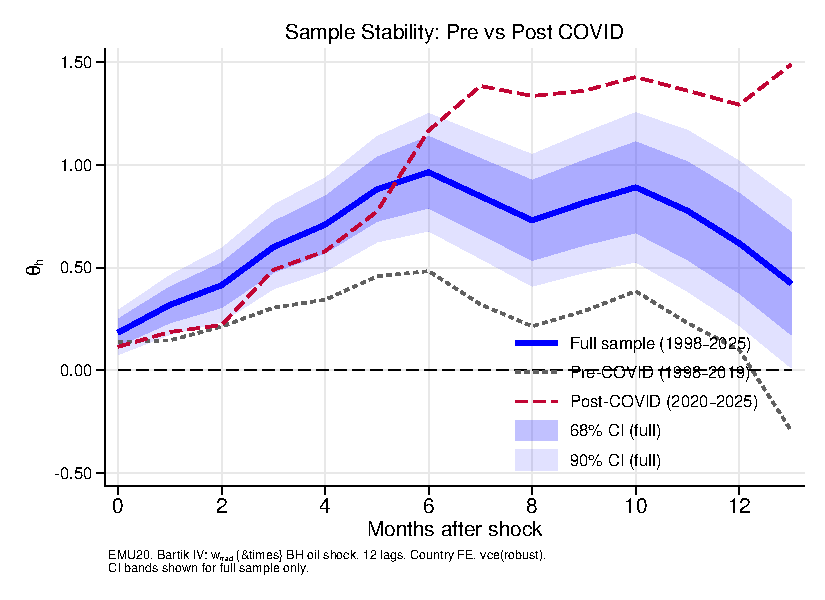
\includegraphics[width=0.85\textwidth]{g_sample_splits.pdf}
    \caption{LP-IV Impulse Responses Across Sample Periods}
    \label{fig:lp_samples}
    \floatfoot{\textit{Note:} Each line reports the response of non-tradable inflation to a one-percentage-point increase in instrumented tradable inflation over different sample periods. Full sample (solid, blue), pre-2020 subsample (short-dashed, grey), and post-2020 subsample (dashed, red). Instrument: Bartik shift-share $Z_{it} = w_{it}\cdot Z_t$. Specification: 12 lags, country fixed effects, EMU20. KP $F$-statistics: full = 208.6, pre-2020 = 132.9, post-2020 = 74.3. Shaded band (full sample only): 90\% confidence interval.}
\end{figure}
\clearpage

\subsection{State-Dependent Pass-Through: The Amplification Mechanism}\label{sec:regimes}

The pre/post-COVID divergence documented in Section~\ref{sec:sample_split} reflects the simultaneous activation of three amplifying regimes during 2020--2023: above-normal supply chain stress, sustained exchange rate depreciation, and elevated inflation volatility. This subsection estimates each regime's independent contribution by splitting the sample along each dimension separately, showing that each condition alone amplifies pass-through by roughly two to four times, and that their joint activation during 2021--2023 provides a coherent structural account of the persistence puzzle.

Whether the second-round pass-through documented above is stable across economic states or amplified in particular conditions is the central question of the regime analysis. Three binary regime indicators partition the estimation sample, and equation~\eqref{eq:lpiv} is re-estimated on each subsample with the same instrument, controls, and fixed effects as the baseline. Estimating separate LP-IVs within each subsample avoids the need for an additional excluded instrument to identify the interaction term $\widehat{\pi^T}_{it}\cdot D_{it}$.

\begin{center}\textcolor{red}{\textbf{[NEED TO ADD REGRESSION SPEC HERE]}} \end{center}

The first dimension captures global supply-chain conditions through the GSCPI of \citeA{BenignodiGiovannietal2022}:
\begin{equation*}
    D^{\mathrm{GSCPI}}_t = \mathbf{1}\bigl[\mathrm{GSCPI}_t > \tilde{q}\bigr],
\end{equation*}
where $\tilde{q}$ denotes the panel median of the GSCPI series; because the index is standardised with mean zero and unit variance, the median threshold is approximately zero, so the high-stress subsample captures episodes of above-normal logistical disruption. The second dimension isolates the direction of the exchange rate:
\begin{equation*}
    D^{\mathrm{NEER}}_{it} = \mathbf{1}\bigl[\Delta\ln\mathrm{NEER}_{it} < 0\bigr],
\end{equation*}
where $D^{\mathrm{NEER}}_{it} = 1$ denotes depreciation months, in which imported cost pressures are amplified relative to appreciation episodes. The third dimension measures the inflation volatility environment:
\begin{equation*}
    D^{\sigma}_{it} = \mathbf{1}\bigl[\hat{\sigma}_{it} > \tilde{\sigma}_i\bigr],
\end{equation*}
where $\hat{\sigma}_{it}$ is the 36-month rolling standard deviation of headline HICP inflation for country $i$ at time $t$, and $\tilde{\sigma}_i$ is the within-country median of that rolling standard deviation; high-volatility periods correspond to episodes of elevated price instability relative to a country's own historical norm.

\autoref{fig:regimes} presents the six impulse responses arranged in a $3\times 2$ panel, with the low-regime subsamples on the left and the high-regime subsamples on the right, with 90 percent confidence intervals shown separately for each.

Along the supply-chain dimension, the contrast between the two subsamples is sharp. During low-GSCPI periods, the response oscillates between 0.1 and 0.5 and the confidence band crosses zero at multiple horizons, leaving the pass-through statistically indistinguishable from zero for much of the window. During high-GSCPI periods, the response rises from 0.33 at impact to a plateau of approximately 1.5 between months six and nine (peak 1.54 at month six), with the 90 percent band lying entirely above zero from month two onward. The near-quadrupling of peak pass-through under supply-chain stress is consistent with the mechanism that logistics disruptions compress firms' substitution margin between imported and domestic inputs, forcing service-sector producers to absorb a larger share of upstream cost shocks rather than switching suppliers; under normal logistical conditions that margin is wider and cost pressures are more readily diversified away. For monetary policy, this finding implies that a central bank that calibrates its response to second-round effects using normal-times estimates will systematically underreact when global supply chains are under stress. GSCPI readings exceeded the panel median for 28 consecutive months between March 2021 and June 2023, placing the entire inflation surge squarely in the high-stress regime.

The exchange rate dimension reveals the most pronounced asymmetry in the dataset. During appreciation episodes ($\Delta\ln\mathrm{NEER}_{it} > 0$), the response is near zero at impact, rises to a modest peak of about 0.7 at month six, and then reverses into negative territory around months eleven through thirteen; the confidence band crosses zero repeatedly and the overall response is statistically indistinguishable from zero across most of the horizon. During depreciation episodes, the picture is entirely different: the response rises strongly from 0.32 at impact to a sustained peak of approximately 2.0 at months ten and eleven, with the confidence band remaining well above zero throughout. The asymmetry is large in magnitude---depreciation pass-through at its peak is roughly three times the appreciation peak---and carries a clear economic interpretation: when the effective exchange rate depreciates, import costs rise in domestic currency terms, amplifying the cost impulse received by non-tradable producers; when it appreciates, the offsetting import-cost relief attenuates or reverses the propagation. From a monetary policy standpoint, this asymmetry implies that exchange rate depreciation episodes sharply amplify the risk of tradable shocks becoming entrenched in domestic service prices, while appreciation provides a natural buffer against such propagation. The euro depreciated against the dollar by approximately 15 percent between January 2021 and September 2022, placing the peak of the inflation episode in the depreciation subsample throughout.

Along the inflation volatility dimension, high-volatility periods display substantially stronger pass-through than low-volatility periods. When inflation volatility is below the within-country median, the response peaks at approximately 0.6 and the confidence band includes zero at several horizons, indicating moderate and imprecisely estimated pass-through. When volatility is above the within-country median, the response rises steeply to a peak of approximately 1.4 at month six and remains above 1.0 through month ten, with the confidence band staying above zero throughout. The pattern is consistent with the view that elevated price instability shortens the effective duration of price contracts and lowers the threshold at which service-sector firms choose to adjust prices, so that a given tradable cost impulse translates into a larger and more immediate adjustment in non-tradable prices. Headline HICP volatility exceeded within-country medians across all EMU member states by mid-2021 and remained elevated through 2023, activating the high-volatility amplification channel for the full duration of the episode.

Taken together, the three amplifying conditions were not independent during the 2021--2023 episode: supply-chain stress raises import input costs that are absorbed more fully when exchange rates depreciate and when the inflation environment is already volatile. The simultaneous activation of all three amplifying regimes explains why post-2020 pass-through reached levels roughly three times the pre-2020 structural estimate documented in Section~\ref{sec:sample_split}, and why aggregate models that ignore regime-switching will systematically underpredict the speed and magnitude of second-round effects during commodity-shock episodes.

\begin{figure}[htbp]
    \centering
    
\includegraphics[width=0.95\textwidth]{g_state_dependence.pdf}
    \caption{State-Dependent LP-IV Impulse Responses of Non-Tradable Inflation}
    \label{fig:regimes}
    \floatfoot{\textit{Note:} Each panel reports the response to a one-percentage-point increase in instrumented tradable inflation within the indicated subsample. Rows correspond to three regime dimensions: global supply-chain pressure (GSCPI above vs.\ below panel median), nominal effective exchange rate direction (appreciation vs.\ depreciation), and inflation volatility (36-month rolling standard deviation of headline HICP above vs.\ below within-country median). Instrument: Bartik shift-share $Z_{it} = w_{it}\cdot Z_t$. Specification: 12 lags, country fixed effects, EMU20 sample (20 countries, January 1998--December 2025). KP $F$-statistics: GSCPI low/high = 98.7/108.2; NEER apprec/deprec = 70.8/126.8; volatility low/high = 146.9/62.3. Shaded bands: 90\% confidence intervals (standard errors clustered at the country level).}
\end{figure}
\clearpage







\subsection{Cross-Country Heterogeneity}\label{sec:heterogeneity}

The EMU20 sample encompasses member states with substantially different structural characteristics. To examine whether second-round pass-through is homogeneous across the union, equation~\eqref{eq:lpiv} is estimated separately for three country groups defined by their structural and historical attributes. The \textit{Core} group (Austria, Belgium, Finland, France, Germany, the Netherlands) comprises the six founding-era economies with relatively low inflation persistence and strong institutional frameworks. The \textit{Periphery} group (Greece, Italy, Portugal, Spain) comprises the four countries with the most troubled fiscal and inflation histories in the post-EMU era. The \textit{Small Open Economies} (SOE) group comprises the remaining ten member states (Croatia, Cyprus, Estonia, Ireland, Latvia, Lithuania, Luxembourg, Malta, Slovakia, Slovenia), which are characterised by high trade openness and, in several cases, currency board histories that precede their euro adoption.

Table~\ref{tab:heterogeneity} reports LP-IV point estimates at selected horizons and pairwise $t$-statistics for group-difference tests. \autoref{fig:heterogeneity} plots the full impulse responses. All three groups yield strong first-stage $F$-statistics (Core: 83.0; Periphery: 36.5; SOE: 112.8), confirming that the Bartik instrument is relevant within each subgroup. The results indicate that pass-through is positive and significant for all three groups throughout the horizon, with the Periphery group displaying the largest estimates: Core and SOE peak at approximately 1.0 at month six, while the Periphery peaks at 1.68. This pattern is consistent with the view that higher historical inflation persistence and weaker inflation-expectation anchoring in peripheral member states amplify the propagation of tradable cost shocks into domestic services. However, Panel~B of Table~\ref{tab:heterogeneity} reveals that no pairwise group difference is statistically significant at the 5~percent level. The maximum absolute $t$-statistic is 1.96 (Periphery versus SOE at $h=0$) and 1.43 (Core versus Periphery at $h=3$). The wide confidence intervals for the Periphery group reflect the small country sample ($N=4$); the directional evidence is economically interpretable but should be treated as suggestive rather than conclusive.

% Phase 5 heterogeneity table — generated by code/8.1_heterogeneity_table.R
\begin{table}[htbp]
\centering
\caption{Second-Round Pass-Through: Heterogeneity Across EMU Groups}
\label{tab:heterogeneity}
{\small
\begin{tabular}{lccc}
\toprule
 & Core & Periphery & Small Open \\
 & (N=6) & (N=4) & (N=10) \\
\midrule
\multicolumn{4}{l}{\textit{Panel A: Point estimates (90\% CI)}} \\[4pt]
$h=0$ & $0.268$ & $0.434$ & $0.124$ \\
      & \footnotesize{$[0.122,\;0.415]$} & \footnotesize{$[0.221,\;0.647]$} & \footnotesize{$[-0.027,\;0.274]$} \\[2pt]
$h=3$ & $0.556$ & $0.999$ & $0.700$ \\
      & \footnotesize{$[0.274,\;0.837]$} & \footnotesize{$[0.575,\;1.422]$} & \footnotesize{$[0.407,\;0.992]$} \\[2pt]
$h=6$ & $1.042$ & $1.678$ & $0.998$ \\
      & \footnotesize{$[0.601,\;1.483]$} & \footnotesize{$[1.003,\;2.354]$} & \footnotesize{$[0.603,\;1.393]$} \\[2pt]
$h=9$ & $0.975$ & $1.164$ & $0.931$ \\
      & \footnotesize{$[0.487,\;1.463]$} & \footnotesize{$[0.429,\;1.900]$} & \footnotesize{$[0.454,\;1.408]$} \\[2pt]
$h=12$ & $0.823$ & $0.963$ & $0.760$ \\
      & \footnotesize{$[0.216,\;1.431]$} & \footnotesize{$[0.145,\;1.781]$} & \footnotesize{$[0.194,\;1.325]$} \\[2pt]
\midrule
\multicolumn{4}{l}{\textit{Panel B: Pairwise group-difference $t$-statistics}} \\[4pt]
 & Core$-$Peri & Core$-$SOE & Peri$-$SOE \\
$h=0$ & $-1.05$ & $1.13$ & $1.96$ \\[2pt]
$h=3$ & $-1.43$ & $-0.58$ & $0.96$ \\[2pt]
$h=6$ & $-1.30$ & $0.12$ & $1.43$ \\[2pt]
$h=9$ & $-0.35$ & $0.11$ & $0.44$ \\[2pt]
$h=12$ & $-0.23$ & $0.13$ & $0.34$ \\[2pt]
\midrule
\multicolumn{4}{l}{\textit{Panel C: First-stage diagnostics}} \\[4pt]
KP $F$-statistic & $83.0$ & $36.5$ & $112.8$ \\
\bottomrule
\end{tabular}
}
\begin{tablenotes}[flushleft]
\footnotesize
\item \textit{Notes:} LP-IV estimates of $\theta_h$ at selected horizons.
Core: DEU, FRA, NLD, AUT, FIN, BEL.
Periphery: ITA, ESP, PRT, GRC.
Small open: IRL, LUX, EST, LVA, LTU, SVK, SVN, MLT, CYP, HRV.
Bartik IV: $Z_{it} = w^{\text{trad}}_{it} \times Z^{\text{BH}}_t$.
Controls: 12 lags of non-tradable inflation, tradable inflation,
unemployment rate, and log NEER change. Country FE. vce(robust).
90\% confidence intervals in brackets.
Panel B: pairwise $t$-statistics under independent samples,
$t = (\hat{\theta}^{g_1}_h - \hat{\theta}^{g_2}_h) \mathbin{/}
\sqrt{\hat{\sigma}^2_{g_1,h} + \hat{\sigma}^2_{g_2,h}}$.
No difference is significant at the 5\% level.
\end{tablenotes}
\end{table}


The country-group results reinforce the state-dependence mechanism identified in Section~\ref{sec:regimes}: the Periphery's structurally larger pass-through implies that the amplification documented in the full-sample regime analysis is likely concentrated in the countries where inflation expectations are least well anchored. For monetary policy in the euro area, this heterogeneity implies that the optimal policy response to a tradable cost shock may need to account not only for the aggregate second-round risk but also for the distribution of that risk across member states with different structural pass-through parameters.

\begin{figure}[htbp]
    \centering
    
\includegraphics[width=0.90\textwidth]{g_lp_heterogeneity.pdf}
    \caption{LP-IV Impulse Responses by EMU Country Group}
    \label{fig:heterogeneity}
    \floatfoot{\textit{Note:} Each line reports the response of non-tradable inflation to a one-percentage-point increase in instrumented tradable inflation for the indicated country group. Core: DEU, FRA, NLD, AUT, FIN, BEL. Periphery: GRC, ITA, ESP, PRT. Small open: IRL, LUX, EST, LVA, LTU, SVK, SVN, MLT, CYP, HRV. Instrument: Bartik shift-share $Z_{it} = w_{it}\cdot Z_t$. Specification: 12 lags, country fixed effects, full EMU20 sample. KP $F$-statistics: Core = 83.0, Periphery = 36.5, SOE = 112.8. Shaded band (Core only): 90\% confidence interval.}
\end{figure}
\clearpage

% %%%%%%%%%%%%%%%%%%%%%%%%%%%%%%%%%%%%%%%%%%%%%%%%%%%%%%%%%%
% %%%%%%%%%%%%%%%%%%%%%%%%%%%%%%%%%%%%%%%%%%%%%%%%%%%%%%%%%%
% Model
% %%%%%%%%%%%%%%%%%%%%%%%%%%%%%%%%%%%%%%%%%%%%%%%%%%%%%%%%%%
% %%%%%%%%%%%%%%%%%%%%%%%%%%%%%%%%%%%%%%%%%%%%%%%%%%%%%%%%%%
\newpage
\section{Model}
\label{sec:model}


% %%%%%%%%%%%%%%%%%%%%%%%%%%%%%%%%%%%%%%%%%%%%%%%%%%%%%%%%%%
% %%%%%%%%%%%%%%%%%%%%%%%%%%%%%%%%%%%%%%%%%%%%%%%%%%%%%%%%%%
% Model
% %%%%%%%%%%%%%%%%%%%%%%%%%%%%%%%%%%%%%%%%%%%%%%%%%%%%%%%%%%
% %%%%%%%%%%%%%%%%%%%%%%%%%%%%%%%%%%%%%%%%%%%%%%%%%%%%%%%%%%
\newpage
\section{Conclusions}
\label{sec:conclusions}

% CONCLUSION TO BE WRITTEN

% %%%%%%%%%%%%%%%%%%%%%%%%%%%%%%%%%%%%%%%%%%%%%%%%%%%%%%%%%%
% %%%%%%%%%%%%%%%%%%%%%%%%%%%%%%%%%%%%%%%%%%%%%%%%%%%%%%%%%%
% REFERENCES SECTION
% %%%%%%%%%%%%%%%%%%%%%%%%%%%%%%%%%%%%%%%%%%%%%%%%%%%%%%%%%%
% %%%%%%%%%%%%%%%%%%%%%%%%%%%%%%%%%%%%%%%%%%%%%%%%%%%%%%%%%%
\newpage
\clearpage
\newpage 
\begin{spacing}{0.9}
\bibliographystyle{apacite}
\bibliography{references}
\end{spacing}

\clearpage



% ==========================
% ==========================
% ==========================
% %%%%%%%%%%%%%%%%%%%%%%%%%%%%%%%%%%%%%%%%%%%%%%%%%%%%%%%%%%
% %%%%%%%%%%%%%%%%%%%%%%%%%%%%%%%%%%%%%%%%%%%%%%%%%%%%%%%%%%
%APPENDIX

% %%%%%%%%%%%%%%%%%%%%%%%%%%%%%%%%%%%%%%%%%%%%%%%%%%%%%%%%%%
% %%%%%%%%%%%%%%%%%%%%%%%%%%%%%%%%%%%%%%%%%%%%%%%%%%%%%%%%%%
% ==========================
% ==========================
% ==========================
\appendix

\setcounter{table}{0}
\renewcommand{\thetable}{\Alph{section}.\arabic{table}}

\setcounter{figure}{0}
\renewcommand{\thefigure}{\Alph{section}.\arabic{figure}}

\begin{center}
    {\LARGE \textbf{When Tradable Inflation Becomes Domestic: Second-Round Effects and Monetary Policy Trade-Offs}} \\
    \vspace{2cm}
    \textbf{Supplemental Appendix} \\
    \vspace{0.2cm}
   \textit{For Online Publication} \\
    \vspace{0.5cm}
    This appendix contains:
\end{center}

\vspace{0.5cm}

\begin{itemize}
    \item \textbf{Appendix A.} Robustness Checks (instrument weight variants; alternative commodity shocks; EU27 extension and EU7 placebo; lag sensitivity)
    \item \textbf{Appendix B.} Full Model of \autoref{sec:model}
    \item \textbf{Appendix C.} Additional Tables and Figures
\end{itemize}

\vfill



\newpage

% ==========================
% %%%%%%%%%%%%%%%%%%%%%%%%%%%%%%%%%%%%%%%%%%%%%%%%%%%%%%%%%%
% %%%%%%%%%%%%%%%%%%%%%%%%%%%%%%%%%%%%%%%%%%%%%%%%%%%%%%%%%%
\newpage
% APPENDIX A
\section{Appendix A. Robustness}
\subsection{Robustness}

\paragraph{Instrument robustness: expenditure-weight variants.}
\autoref{fig:lp_rob_w} compares the baseline Bartik instrument against two alternatives: a Bartik scaled by import exposure ($w^{\mathrm{imp}}_{it} = \mathrm{imports}/\mathrm{GDP}$) and the unscaled market-based oil price shock $Z_t$ used directly without country-level weighting. The import-exposure Bartik captures a different dimension of openness, the share of domestic expenditure that is sourced from abroad, while the unscaled instrument exploits only the common time-series variation in $Z_t$ and relies on country fixed effects to absorb permanent differences in exposure. Ninety-percent confidence intervals are shown for the baseline specification only. The three-point estimate paths are virtually indistinguishable across the entire twelve-month horizon: all three rise together from approximately 0.18 at impact to peaks near 0.96 at month six, with the import-to-GDP Bartik and the unscaled shock tracking the baseline so closely that the lines are nearly superimposed throughout. This near-perfect agreement across instruments that exploit different sources of cross-country heterogeneity strongly supports the conclusion that the pass-through estimate is not an artifact of any particular exposure weighting.

\begin{figure}[ht]
    \centering
    
\includegraphics[width=0.85\textwidth]{g_lp_base_rob_w.pdf}
    \caption{LP-IV Impulse Responses Under Alternative Bartik Weight Specifications}
    \label{fig:lp_rob_w}
    \floatfoot{\textit{Note:} Each line reports the response of non-tradable inflation to a one-percentage-point increase in instrumented tradable inflation under a different instrument specification. Baseline (solid, blue): Bartik instrument $Z_{it} = w_{it}\cdot Z_t$, where $w_{it}$ is the tradables expenditure share. Robustness 1 (dashed, red): Bartik scaled by import-to-GDP ratio, $Z_{it} = (m_{it}/y_{it})\cdot Z_t$. Robustness 2 (short-dashed, grey): unscaled oil price shock $Z_t$. Specification: 12 lags, country fixed effects, pre-2020 sample. Shaded band (baseline only): 90\% confidence interval.}
\end{figure}
\clearpage

\paragraph{Instrument robustness: alternative commodity shocks.}
\autoref{fig:lp_rob_instruments} and Table~\ref{tab:rob_instruments} compare the baseline Baumeister--Hamilton oil price expectation shock against the IMF non-fuel primary commodity price index, processed as an AR(1) innovation on log-differences. Both instruments yield strong first stages: KP $F$-statistics of 208.6 (BH) and 176.1 (IMF), well above any weak-instrument threshold. The qualitative shape of the impulse response is confirmed under both: positive throughout, peaking around month six with a secondary hump near month ten. However, the IMF non-fuel estimates are systematically larger, peaking at 1.98 at month six and continuing to rise to 2.78 at month twelve, compared to the BH peak of 0.96 at month six. This divergence is economically interpretable: the IMF basket aggregates agricultural commodities and metals alongside energy-related tradables, capturing a broader set of tradable cost pressures that transmit through additional channels (food and material costs) and with longer lags. The BH estimate should therefore be interpreted as a conservative, oil-channel-specific lower bound, while the IMF estimate provides the upper end of the commodity price transmission channel. The GSCPI instrument (AR(2) innovations on the NY Fed Global Supply Chain Pressure Index) was excluded at the estimation stage due to a near-zero first-stage $F$-statistic ($\approx 2$), far below the Stock--Yogo critical value of 16.38; full documentation of this failure is provided in Table~\ref{tab:rob_instruments}.

\begin{figure}[ht]
    \centering
    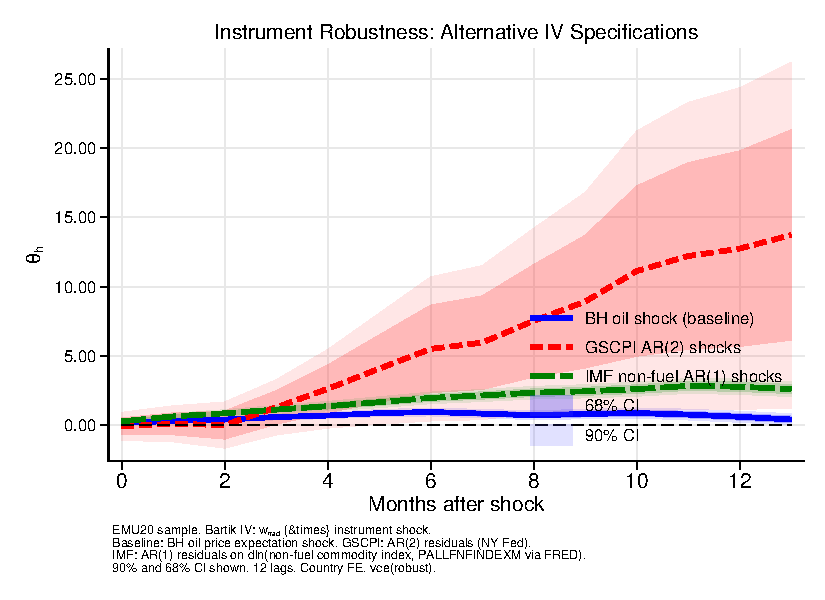
\includegraphics[width=0.85\textwidth]{g_lp_rob_instruments.pdf}
    \caption{LP-IV Impulse Responses Under Alternative Commodity Shock Instruments}
    \label{fig:lp_rob_instruments}
    \floatfoot{\textit{Note:} Baseline (solid, blue): Bartik IV using BH oil price expectation shock. Alternative (dashed, red): Bartik IV using AR(1) innovations on IMF non-fuel commodity index (PALLFNFINDEXM). Specification: 12 lags, country fixed effects, EMU20, full sample. KP $F$: BH = 208.6, IMF = 176.1. Shaded band (BH only): 90\% confidence interval.}
\end{figure}

% Phase 4 instrument robustness table — generated by code/7.2_rob_instruments_table.R
\begin{table}[htbp]
\centering
\caption{Instrument Robustness: Alternative IV Specifications}
\label{tab:rob_instruments}
{\small
\begin{tabular}{lcc}
\toprule
 & BH Oil Shock & IMF Non-Fuel \\
 & (Baseline) & Commodity Shock \\
\midrule
\multicolumn{3}{l}{\textit{Panel A: Point estimates (90\% CI)}} \\[4pt]
$h=0$ & $0.184$ & $0.293$ \\
      & \footnotesize{$[0.076,\;0.291]$} & \footnotesize{$[0.157,\;0.429]$} \\[2pt]
$h=3$ & $0.600$ & $1.136$ \\
      & \footnotesize{$[0.397,\;0.803]$} & \footnotesize{$[0.834,\;1.437]$} \\[2pt]
$h=6$ & $0.964$ & $1.982$ \\
      & \footnotesize{$[0.678,\;1.249]$} & \footnotesize{$[1.565,\;2.399]$} \\[2pt]
$h=9$ & $0.815$ & $2.455$ \\
      & \footnotesize{$[0.476,\;1.155]$} & \footnotesize{$[1.980,\;2.929]$} \\[2pt]
$h=12$ & $0.618$ & $2.783$ \\
      & \footnotesize{$[0.219,\;1.017]$} & \footnotesize{$[2.227,\;3.339]$} \\[2pt]
\midrule
\multicolumn{3}{l}{\textit{Panel B: First-stage diagnostics}} \\[4pt]
KP $F$-statistic & $208.6$ & $176.1$ \\
Countries & 20 & 20 \\
\bottomrule
\end{tabular}
}
\begin{tablenotes}[flushleft]
\footnotesize
\item \textit{Notes:} LP-IV estimates of the tradable-to-non-tradable
inflation pass-through coefficient $\theta_h$ at selected horizons.
EMU20 sample. Bartik IV: $Z_{it} = w^{\text{trad}}_{it} \times \text{shock}_t$.
BH: Baumeister-Hamilton oil price expectation shock.
IMF: AR(1) innovations on log-differences of the IMF non-fuel primary
commodity price index (PALLFNFINDEXM via FRED).
Controls: 12 lags of non-tradable inflation, tradable inflation,
unemployment rate, and log NEER change. Country FE. vce(robust).
90\% confidence intervals in brackets.
GSCPI instrument (AR(2) innovations on the NY Fed Global Supply Chain
Pressure Index, both Bartik-weighted and direct) excluded: KP $F < 4$
in all specifications (weak instrument). BDI: unavailable.
\end{tablenotes}
\end{table}


\clearpage

\paragraph{Sample extension: EU27 and EU7 placebo.}
\autoref{fig:lp_eu27} and Table~\ref{tab:phase3_comparison} examine whether the EMU20 result replicates on extended samples. The EU27 specification adds the seven non-EMU EU member states (Bulgaria, Czech Republic, Denmark, Hungary, Poland, Romania, Sweden) and uses the bilateral EUR spot rate as the NEER measure for those countries. The EU7 placebo estimates the same specification on non-EMU EU members alone, which should---if the identification strategy is clean---produce insignificant pass-through absent a monetary policy commitment to the euro.

The EU27 result closely mirrors the EMU20 baseline (peak 0.887 at month six, KP $F = 230.5$), confirming that second-round pass-through is present across the broader EU. The EU7 placebo, however, does not fully confirm absence of pass-through: the response is insignificant at months zero to five but rises to significance at months seven to twelve, peaking at 1.23 at month twelve. Two mechanisms plausibly explain this: Bulgaria and Denmark operate de facto EUR pegs, and several Central and Eastern European economies have deep EUR-invoiced trade linkages that produce delayed transmission. The EU7 comparison should therefore be interpreted with caution rather than as a clean falsification test; the EMU-specific identification narrative rests primarily on the Bartik instrument's cross-sectional variation within the EMU rather than on the EU7 comparison.

\begin{figure}[ht]
    \centering
    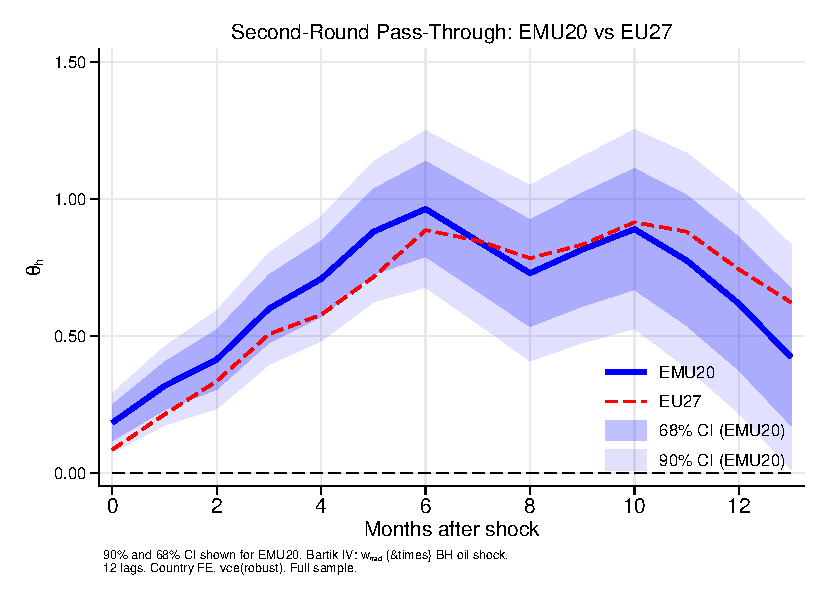
\includegraphics[width=0.85\textwidth]{g_lp_eu27_comparison.pdf}
    \caption{LP-IV Impulse Responses: EMU20 vs.\ EU27 Extension}
    \label{fig:lp_eu27}
    \floatfoot{\textit{Note:} EMU20 (solid, blue) versus EU27 (dashed, red). EU27 adds BG, CZ, DK, HU, PL, RO, SE; NEER for non-EMU countries uses bilateral EUR spot rate. Instrument: Bartik shift-share $Z_{it} = w_{it}\cdot Z_t$. Specification: 12 lags, country fixed effects, full sample. KP $F$: EMU20 = 208.6, EU27 = 230.5. Shaded band (EMU20 only): 90\% confidence interval.}
\end{figure}

\begin{figure}[ht]
    \centering
    
\includegraphics[width=0.85\textwidth]{g_lp_emu20_vs_eu7.pdf}
    \caption{LP-IV Impulse Responses: EMU20 vs.\ EU7 Placebo}
    \label{fig:lp_eu7}
    \floatfoot{\textit{Note:} EMU20 (solid, blue) versus EU7 placebo (dashed, red, non-EMU EU countries only). EU7 countries: BG, CZ, DK, HU, PL, RO, SE. The EU7 placebo is not a clean falsification test due to EUR-pegged countries (BG, DK) and deep EUR trade linkages in CEE. Instrument: Bartik shift-share $Z_{it} = w_{it}\cdot Z_t$. Specification: 12 lags, country fixed effects. KP $F$: EU7 = 50.3. Shaded band (EMU20 only): 90\% confidence interval.}
\end{figure}

% Phase 3 comparison table — generated by code/6.3_phase3_table.R
\begin{table}[htbp]
\centering
\caption{Second-Round Pass-Through: Baseline Replication and EU27 Extension}
\label{tab:phase3_comparison}
{\small
\begin{tabular}{lccc}
\toprule
 & EMU20 & EU27 & EU7 Placebo \\
\midrule
\multicolumn{4}{l}{\textit{Panel A: Point estimates (90\% CI)}} \\[4pt]
$h=0$ & $0.184$ & $0.085$ & $-0.175$ \\
      & \footnotesize{$[0.076,\;0.291]$} & \footnotesize{$[-0.032,\;0.203]$} & \footnotesize{$[-0.434,\;0.084]$} \\[2pt]
$h=3$ & $0.600$ & $0.507$ & $0.229$ \\
      & \footnotesize{$[0.397,\;0.803]$} & \footnotesize{$[0.313,\;0.701]$} & \footnotesize{$[-0.200,\;0.658]$} \\[2pt]
$h=6$ & $0.964$ & $0.887$ & $0.669$ \\
      & \footnotesize{$[0.678,\;1.249]$} & \footnotesize{$[0.619,\;1.155]$} & \footnotesize{$[0.068,\;1.269]$} \\[2pt]
$h=9$ & $0.815$ & $0.833$ & $0.983$ \\
      & \footnotesize{$[0.476,\;1.155]$} & \footnotesize{$[0.512,\;1.155]$} & \footnotesize{$[0.268,\;1.697]$} \\[2pt]
$h=12$ & $0.618$ & $0.743$ & $1.231$ \\
      & \footnotesize{$[0.219,\;1.017]$} & \footnotesize{$[0.370,\;1.117]$} & \footnotesize{$[0.406,\;2.057]$} \\[2pt]
\midrule
\multicolumn{4}{l}{\textit{Panel B: First-stage diagnostics}} \\[4pt]
KP $F$-statistic & $208.6$ & $230.5$ & $50.3$ \\
Countries & 20 & 27 & 7 \\
\bottomrule
\end{tabular}
}
\begin{tablenotes}[flushleft]
\footnotesize
\item \textit{Notes:} LP-IV estimates of the tradable-to-non-tradable
inflation pass-through coefficient $\theta_h$ at selected horizons.
Bartik IV: $Z_{it} = w^{\text{trad}}_{it} \times Z^{\text{BH}}_t$.
Controls: 12 lags of non-tradable inflation, tradable inflation,
unemployment rate, and log NEER change. Country FE. vce(robust).
90\% confidence intervals in brackets. KP $F$-statistic uniform
across horizons by construction of the Bartik instrument.
EU7 NEER: bilateral EUR spot rate (ECB EXR).
\end{tablenotes}
\end{table}


\clearpage

\paragraph{Lag sensitivity.}
\autoref{fig:lag_sensitivity} examines sensitivity to the number of control lags $L \in \{4, 8, 12, 16\}$. The choice of 12 lags in the baseline follows the conventional rule for monthly data. Across all four specifications the shape of the impulse response is stable: all four paths track closely from impact through month thirteen, with the peak at month six ranging from 0.88 ($L=16$) to 1.04 ($L=4$). The Kleibergen--Paap $F$-statistic increases with more lags (169 to 255), reflecting tighter conditioning on pre-sample history. These results confirm that the baseline pass-through profile is not sensitive to the lag length choice within the range considered in the monthly VAR literature.

\begin{figure}[ht]
    \centering
    
\includegraphics[width=0.85\textwidth]{g_lag_sensitivity.pdf}
    \caption{LP-IV Impulse Responses Under Alternative Lag Lengths}
    \label{fig:lag_sensitivity}
    \floatfoot{\textit{Note:} Each line reports the response under $L \in \{4, 8, 12, 16\}$ control lags. Instrument: Bartik shift-share $Z_{it} = w_{it}\cdot Z_t$. Specification: country fixed effects, EMU20, full sample. KP $F$-statistics: $L=4$: 168.5; $L=8$: 184.4; $L=12$: 208.6; $L=16$: 254.8.}
\end{figure}
\clearpage


% %%%%%%%%%%%%%%%%%%%%%%%%%%%%%%%%%%%%%%%%%%%%%%%%%%%%%%%%%%
% %%%%%%%%%%%%%%%%%%%%%%%%%%%%%%%%%%%%%%%%%%%%%%%%%%%%%%%%%%
\newpage
% Appendix B
\section{Appendix B. Full Model of \autoref{sec:model}}

% ==========================
% %%%%%%%%%%%%%%%%%%%%%%%%%%%%%%%%%%%%%%%%%%%%%%%%%%%%%%%%%%
% %%%%%%%%%%%%%%%%%%%%%%%%%%%%%%%%%%%%%%%%%%%%%%%%%%%%%%%%%%
% APPENDIX C TABLES
\newpage
\section{Appendix C. Additional tables and figures}

% %%%%%%%%%%%%%%%%%%%%%%%%%%%%%%%%%%%%%%%%%%%%%%%%%%%%%%%%%%
% %%%%%%%%%%%%%%%%%%%%%%%%%%%%%%%%%%%%%%%%%%%%%%%%%%%%%%%%%%
% SUMMARY STATISTICS
\begin{table}[htbp]
  \centering
  \begin{threeparttable}
  \caption{Summary Statistics}
  \label{tab:summary}
  \footnotesize
  \begin{tabular*}{\textwidth}{@{\extracolsep{\fill}}lrrrrr}
    \toprule
    Variable & $N$ & Mean & Std.\ Dev. & Min & Max \\
    \midrule
    Headline inflation & 6,372 & 2.67 & 2.85 & -4.35 & 25.16 \\
    Tradable inflation & 6,372 & 2.48 & 3.01 & -4.09 & 22.02 \\
    Non-tradable inflation & 6,337 & 2.96 & 3.30 & -7.04 & 36.63 \\
    Market oil price shock & 5,776 & 0.01 & 0.05 & -0.32 & 0.09 \\
    Oil supply shock & 6,327 & -0.13 & 1.24 & -10.86 & 3.56 \\
    GSCPI & 6,384 & 0.01 & 1.00 & -1.58 & 4.48 \\
    $\Delta \ln$ NEER & 6,384 & 0.10 & 1.31 & -3.92 & 5.21 \\
    Unemployment rate (\%) & 6,284 & 8.36 & 3.97 & 1.80 & 26.40 \\
    IP growth, YoY (\%) & 5,568 & 2.02 & 8.43 & -44.05 & 79.25 \\
    Import exposure (\% of GDP) & 6,192 & 61.46 & 29.61 & 21.00 & 189.90 \\
    \bottomrule
  \end{tabular*}
  \begin{tablenotes}
    \footnotesize
    \item \textit{Note:} Inflation rates are year-over-year percent changes. GSCPI is standardized with a mean of zero and unit variance. NEER change and oil shocks are in log points. Sample: 20 euro area countries (EMU20), January 1998 -- December 2025.
  \end{tablenotes}
  \end{threeparttable}
\end{table}

% %%%%%%%%%%%%%%%%%%%%%%%%%%%%%%%%%%%%%%%%%%%%%%%%%%%%%%%%%%
% %%%%%%%%%%%%%%%%%%%%%%%%%%%%%%%%%%%%%%%%%%%%%%%%%%%%%%%%%%
% DATA SOURCES
\begin{landscape}
    
\begin{table}[htbp]
  \centering
  \caption{Data Sources}
  \label{tab:sources}
  \begin{tabular}{llp{5cm}}
    \toprule
    Variable & Description & Source \\
    \midrule
    \texttt{pi\_headline} & Headline HICP inflation (YoY, \%) & Eurostat \texttt{prc\_hicp\_midx} \\
    \texttt{pi\_trad} & Tradable inflation, Eq.~(\ref{eq:basket}), $\mathcal{B}=\mathcal{T}$ & Authors' construction \\
    \texttt{pi\_nontrad} & Non-tradable inflation, Eq.~(\ref{eq:basket}), $\mathcal{B}=\mathcal{N}$ & Authors' construction \\
    \texttt{w\_food}, \texttt{w\_clothing}, \ldots & Annual ECOICOP expenditure weights (normalized) & Eurostat \texttt{prc\_hicp\_inw} \\
    \texttt{bh\_oil\_price\_exp\_shock} & Market-based oil price expectation shock & \shortciteA{BaumeisterHamilton2019} \\
    \texttt{bh\_oil\_supply\_shock} & Structural oil supply shock & \citeA{BaumeisterHamilton2019} \\
    \texttt{gscpi} & Global Supply Chain Pressure Index & \shortciteA{BenignodiGiovannietal2022} \\
    \texttt{dln\_neer} & Log monthly change in nominal effective exchange rate & ECB Data Portal API \\
    \texttt{ur} & Unemployment rate, seasonally adjusted (\% of active population) & Eurostat \texttt{une\_rt\_m} \\
    \texttt{ip\_gr\_yoy} & Manufacturing IP growth, year-over-year (\%) & Eurostat \texttt{sts\_inpr\_m} \\
    \texttt{wi\_imp\_gdp} & Imports of goods and services (\% of GDP) & Eurostat \texttt{nama\_10\_gdp} \\
    \midrule
    \multicolumn{3}{l}{\footnotesize\textit{Note:} ECOICOP tradable basket $\mathcal{T}$: CP01, CP02, CP03, CP05, CP07. Non-tradable basket $\mathcal{N}$: CP04, CP06, CP08, CP09, CP10, CP11, CP12.}\\
    \bottomrule
  \end{tabular}
\end{table}
\end{landscape}

% %%%%%%%%%%%%%%%%%%%%%%%%%%%%%%%%%%%%%%%%%%%%%%%%%%%%%%%%%%
% %%%%%%%%%%%%%%%%%%%%%%%%%%%%%%%%%%%%%%%%%%%%%%%%%%%%%%%%%%
% COUNTRY COVERAGE
\begin{table}[htbp]
  \centering
  \begin{threeparttable}
  \caption{Country Coverage}
  \label{tab:coverage}
  \footnotesize
  \begin{tabular*}{\textwidth}{@{\extracolsep{\fill}}llccc}
    \toprule
    Country & ISO & Start & End & $N$ \\
    \midrule
    Austria     & AUT & 1998m01 & 2025m12 & 336 \\
    Belgium     & BEL & 1998m01 & 2025m12 & 336 \\
    Croatia     & HRV & 1999m01 & 2025m12 & 324 \\
    Cyprus      & CYP & 1998m01 & 2025m12 & 336 \\
    Estonia     & EST & 1998m01 & 2025m12 & 336 \\
    Finland     & FIN & 1998m01 & 2025m12 & 336 \\
    France      & FRA & 1998m01 & 2025m12 & 336 \\
    Germany     & DEU & 1998m01 & 2025m12 & 336 \\
    Greece      & GRC & 1998m01 & 2025m12 & 336 \\
    Ireland     & IRL & 1998m01 & 2025m12 & 336 \\
    Italy       & ITA & 1998m01 & 2025m12 & 336 \\
    Latvia      & LVA & 1998m01 & 2025m12 & 336 \\
    Lithuania   & LTU & 1998m01 & 2025m12 & 336 \\
    Luxembourg  & LUX & 1998m01 & 2025m12 & 336 \\
    Malta       & MLT & 1998m01 & 2025m12 & 336 \\
    Netherlands & NLD & 1998m01 & 2025m12 & 336 \\
    Portugal    & PRT & 1998m01 & 2025m12 & 336 \\
    Slovakia    & SVK & 1998m01 & 2025m12 & 336 \\
    Slovenia    & SVN & 1998m01 & 2025m12 & 336 \\
    Spain       & ESP & 1998m01 & 2025m12 & 336 \\
    \bottomrule
  \end{tabular*}
  \begin{tablenotes}
    \footnotesize
    \item \textit{Note:} $N$ counts non-missing observations of headline HICP inflation. Sample: 20 euro area member states (EMU20), January 1998 -- December 2025.
  \end{tablenotes}
  \end{threeparttable}
\end{table}


% %%%%%%%%%%%%%%%%%%%%%%%%%%%%%%%%%%%%%%%%%%%%%%%%%%%%%%%%%%
% %%%%%%%%%%%%%%%%%%%%%%%%%%%%%%%%%%%%%%%%%%%%%%%%%%%%%%%%%%




\clearpage


\end{document}